% ---- Modele TP PC V2 -----------
\documentclass[a4paper,9pt,french]{scrartcl}
\usepackage[T1]{fontenc}
\usepackage{array}
\usepackage{titlesec}
\usepackage{ulem}
\usepackage[dvipsnames]{xcolor}
\usepackage{color}
\usepackage{babel}

\usepackage{graphicx}
\usepackage[utf8]{inputenc}
\usepackage{geometry}
\usepackage{tikz}
\usepackage{fancyhdr}
\usepackage{hyperref}
\usepackage{caption}
 \usepackage{float}
 \usepackage{multicol}
 \usepackage{amsmath}
 \usepackage{amssymb}
 \geometry{vmargin=2.5cm}

\captionsetup{labelfont=sc}
\def\frenchtablename{Tableau}
\pagestyle{fancy}
\renewcommand\headrulewidth{1pt}
\fancyhead[L]{TP II - Moteur à air chaud}
\fancyhead[R]{Saux Paulhenry}
\title{Étude thermodynamique d'un moteur ditherme à récupérateur}
\date{\today}
\author{}

\geometry{a4paper}

\makeatletter
\newcommand{\coloruline}[2]{%
        \UL@protected\def\temp@uline{\leavevmode \bgroup
            \markoverwith{\textcolor{#1}{\rule[-0.5ex]{2pt}{0.4pt}}}%
        \ULon}%
        \temp@uline{#2}%
    }
    \newcommand{\coloruuline}[2]{%
        \UL@protected\def\temp@uuline{\leavevmode \bgroup
            \UL@setULdepth
            \ifx\UL@on\UL@onin \advance\ULdepth2.8\p@\fi
            \markoverwith{\textcolor{#1}{\lower\ULdepth\hbox
                {\kern-.03em\vbox{\hrule width.2em\kern1\p@\hrule}\kern-.03em}}}%
        \ULon}%
        \temp@uuline{#2}%
    }
\makeatother

\renewcommand{\thesection}{\arabic{section}}
\renewcommand{\thesubsection}{\arabic{subsection}}
\renewcommand{\thesubsubsection}{\arabic{subsubsection}}

\begin{document}

% ---------------- Modification des titres --------------------
\titleformat{\section}{\Large}{\coloruuline{red}{\thesection. }}{0ex}{\coloruuline{red}}[]
\titleformat{\subsection}{\Large}{\coloruline{red}{\thesection.\thesubsection. }}{0ex}{\coloruline{red}}[]
\titleformat{\subsubsection}{\large}{\coloruline{ForestGreen}{\thesection.\thesubsection.\thesubsubsection. }}{0ex}{\coloruline{ForestGreen}}[]
\section{Introduction}
\subsection{Objectifs}
Ce TP vise à étudier le fonctionnement d'un moteur thermique ditherme à air chaud. Les objectifs sont :
\begin{itemize}
    \item Analyse qualitativement du cycle du moteur et comprendre le rôle du régénérateur.
    \item La mesure expérimentale avec CassyLab du travail $W$ et des transferts thermiques $Q_c$ et $Q_f$.
    \item Le calcul de l'efficacité énergétique réelle $\eta_M$ et sa comparaison avec les modèles théoriques.
\end{itemize}

\subsection{Sommaire}
Le TP se décompose en 2 parties
\begin{enumerate}
 \item Analyse qualitative et description du cycle.
 \item Analyse quantitative puis bilan énergétique et calcul d'efficacité.
\end{enumerate}

\section{Protocole}
\subsection{Matériel}
L'installation comprend un cylindre vertical en verre, un piston en acier ($A = 28,3$ cm$^2$), un régénérateur poreux en cuivre, un filament chauffant (effet Joule) et un circuit de refroidissement à eau. L'acquisition est réalisée via le système CASSY.

\subsection{Description du montage expérimental}

Le fluide caloporteur est l'air contenu dans le cylindre (système fermé). Le régénérateur se déplace pour confiner l'air soit vers la source chaude (haut), soit vers la source froide (bas). Le déphasage entre le mouvement du régénérateur et celui du piston permet la production de travail.

\begin{figure}[H]
 \begin{center}

\includegraphics[scale=0.4]{schema.pdf}
 \end{center}
\caption{ Représentation d'un cycle}
\end{figure}

\subsection{Mesures à effectuer}
\begin{itemize}
    \item Calibration : Relevé de $s_0$ (position pour $V_{min} = 195$ cm$^3$). On place le moteur de façon à ce que le piston soit le plus bas possible.
    \item Acquisition de $p_{rel}(t)$ et $s(t)$.
    \item Mesure du débit d'eau $D_v$ et des températures $T_{entrée}$, $T_{sortie}$.
    \item Mesure de $U$ et $I$ du filament.
\end{itemize}
\section{Analyse qualitative}

\subsection{Mise en service et identification des composants}
La partie moteur se décompose en trois éléments clés :
\begin{itemize}
    \item {Le cylindre et le piston :} Ils délimitent le volume $V$ du système fermé (l'air). Le piston assure la conversion de l'énergie de pression en travail mécanique.
    \item {Le filament métallique :} Situé en partie haute, il joue le rôle de {source chaude} par dissipation d'énergie Joule.
    \item {Le régénérateur :} Pièce mobile poreuse en cuivre située à l'intérieur du cylindre. Son rôle est de déplacer l'air entre la zone chaude et la zone froide. L'air ne passe pas autour du régénérateur (car il y a un joint d'étanchéité), mais il passe à travers lui, par le milieu poreux en cuivre.
    Ainsi, de haut en bas : L'air arrive chaud, traverse le cuivre, lui donne sa chaleur, et ressort moins chaud en bas. Le cuivre "stocke" cette énergie.
    À l'inverse, de bas en haut : L'air arrive froid, traverse le cuivre encore chaud, récupère l'énergie stockée, et ressort déjà préchauffé en haut. L'un dans l'autre, les contibutions énergétiques du régénérateur au système s'annulent.

\end{itemize}

\subsection{Étude cinématique du cycle}
En faisant tourner le volant d'inertie manuellement dans le sens horaire, on décompose le mouvement en quatre phases distinctes basées sur les positions relatives du piston et du régénérateur :

\begin{enumerate}
    \item {Compression :} Le régénérateur est en position haute, maintenant l'air dans la partie inférieure du cylindre (zone froide). Le piston remonte, comprimant l'air à basse température. Cette phase consomme du travail, fourni par l'inertie du volant. Comme la pression est faible (air froid), ce travail est minimal.
    
    \item {Transfert vers le chaud :} Le piston est au point mort haut. Le régénérateur descend vers le piston, forçant l'air froid à traverser sa structure poreuse vers le haut (zone chaude). En circulant, l'air récupère l'énergie thermique stockée dans le cuivre du régénérateur et se préchauffe avant d'atteindre le filament.
    
    \item {Détente (Expansion) :} Le régénérateur est maintenant en position basse, confinant l'air en haut au contact du filament (source chaude). L'air s'échauffe brutalement, sa pression augmente fortement et repousse le piston vers le bas. Le système fournit alors un travail moteur important au volant d'inertie.
    
    \item {Transfert vers le froid :} Le piston est au point mort bas. Le régénérateur remonte vers le haut du cylindre, chassant l'air chaud vers la partie inférieure refroidie par l'eau. En traversant le régénérateur, l'air cède sa chaleur au cuivre (stockage thermique) et arrive refroidi dans la zone inférieure, prêt pour un nouveau cycle.
\end{enumerate}

\subsection{Inversion du sens de rotation}

En inversant le sens de rotation du volant, on modifie le déphasage entre le piston et le régénérateur. 
\begin{enumerate}
    \item {Phase 1 - Détente à froid :} Contrairement au mode moteur, le volume augmente (le piston descend) alors que le régénérateur est en position haute, maintenant l'air dans la zone inférieure (source froide). La détente du gaz provoque une chute de sa température en dessous de celle de l'eau de refroidissement, permettant au gaz d'absorber de la chaleur à la source froide.
    
    \item {Phase 2 - Transfert vers le chaud :} Le régénérateur descend alors que le piston est en position basse. L'air froid est poussé vers la partie supérieure. En traversant le milieu poreux, il capte l'énergie thermique résiduelle, mais arrive dans une zone déjà portée à haute température par le filament\footnote{C'est pour cela qu'il faut faire tourner le moteur dans le bon sens, afin d'éviter d'endommager le filament.}.
    
    \item {Phase 3 - Compression à chaud :} Le piston remonte (diminution de volume) alors que l'air est maintenu en haut par le régénérateur en position basse. La compression mécanique augmente la température du gaz au-delà de celle de la source chaude. Le fluide cède alors de la chaleur au filament (ou à l'enceinte supérieure).
    
    \item {Phase 4 - Transfert vers le froid :} Le régénérateur remonte, chassant l'air comprimé vers la zone inférieure. En traversant le cuivre, le gaz cède une grande partie de son énergie thermique au régénérateur avant de recommencer un cycle de détente.
\end{enumerate}
Le système consomme du travail mécanique pour forcer un transfert thermique de la source froide vers la source chaude. Le dispositif agit alors comme la {machine frigorifique}.
\subsection{Bilan énergétique qualitatif}
En régime permanent, les échanges d'énergie entre l'air et son environnement sont les suivants :
\begin{itemize}
    \item {Travail ($W$) :} Échangé avec le piston. Le travail net sur un cycle est négatif ($W < 0$), le système est moteur.
    \item {Chaleur avec la source chaude ($Q_C > 0$) :} Reçue au niveau du filament en haut du cylindre.
    \item {Chaleur avec la source froide ($Q_F < 0$) :} Cédée à l'eau de refroidissement en bas du cylindre.
    \item {Échanges avec le régénérateur :} Le régénérateur reçoit de la chaleur lors du transfert chaud $\to$ froid et la restitue lors du transfert froid $\to$ chaud. Sur un cycle complet, la quantité d'énergie reçue par le régénérateur est donc considérée comme nulle.
\end{itemize}

\subsection{Synthèse du principe de fonctionnement}
Le moteur produit un travail continu grâce au déphasage entre le mouvement du piston et celui du régénérateur. En déplaçant la masse d'air de façon cyclique entre une zone où elle se détend à haute pression (température élevée) et une zone où elle est compressée à basse pression (basse température), le travail de détente fourni par le gaz est supérieur au travail de compression qu'il faut lui apporter. L'utilisation du régénérateur  
permet de "recycler" une partie de l'énergie interne du gaz,ce qui augmente l'efficacité thermique du moteur.
\section{Mesures}
\subsection{Données expérimentales}
\begin{table}[H]
\centering
\begin{tabular}{|l|c|r|}
\hline
Grandeur & Symbole & Valeur (Exemple) \\ \hline
Pression atmosphérique & $P_{atm}$ & $1013 \pm 1$ hPa \\
Position volume min & $s_0$ & $4.76 \pm 0,01$ cm \\
Courant filament & $I$ & $11,5 \pm 0,1$ A \\
Tension filament & $U$ & $12.2 \pm 0,1$ V \\
Débit d'eau & $D_v$ & $4.39 \cdot 10^{-6}$ m$^3$/s \\
\hline
\end{tabular}
\caption{Synthèse des paramètres expérimentaux}
\end{table}
\subsection{Détermination du débit massique d'eau}
Le débit volumique $D_v$ est mesuré par chronométrage d'un volume $V = 500$ mL à la sortie du circuit de refroidissement. 

\begin{itemize}
    \item $V_{eau} = 500 \cdot 10^{-6}$ m$^3$ 
    \item $\Delta t = 113,91$ s (soit 1 min 53,91 s)
\end{itemize}

Le débit volumique en unités SI est :
$$D_v = \frac{V_{eau}}{\Delta t} = 4,39 \cdot 10^{-6} \text{ m}^3\text{.s}^{-1}$$
Le débit massique $D_m$ s'en déduit (avec $\rho_{eau} = 1000$ kg.m$^{-3}$) :
$$D_m = \rho_{eau} \cdot D_v = 4,39 \cdot 10^{-3} \text{ kg.s}^{-1}$$



\subsection{Incertitudes}
L'incertitude sur le volume est donnée par :
$u(V) = \sqrt{u(V_0)^2 + A^2 u(s)^2 + (s-s_0)^2 u(A)^2}$.
L'incertitude sur la puissance thermique cédée à l'eau est :
$\frac{u(P_F)}{P_F} = \sqrt{\left(\frac{u(D_v)}{D_v}\right)^2 + \frac{u(\Delta T)^2}{\Delta T^2}}$.
\subsubsection{Débit volumique}
Avec une erreur estimée de $u(V) = 5$ mL (due à la précision des graduations du becher) et $u(t) = 0,2$ s (du à la réactivité du chronométreur), l'incertitude relative est dominée par la précision de l'éprouvette ($1\%$) :
$$u(D_m) = D_m \cdot \sqrt{\left(\frac{u(V)}{V}\right)^2 + \left(\frac{u(t)}{t}\right)^2} \approx 0,04 \cdot 10^{-3} \text{ kg.s}^{-1}$$
On obtient $D_m = (4,39 \pm 0,04) \cdot 10^{-3}$ kg.s$^{-1}$
\section{Graphiques}
\begin{figure}[H]
    \begin{center}
        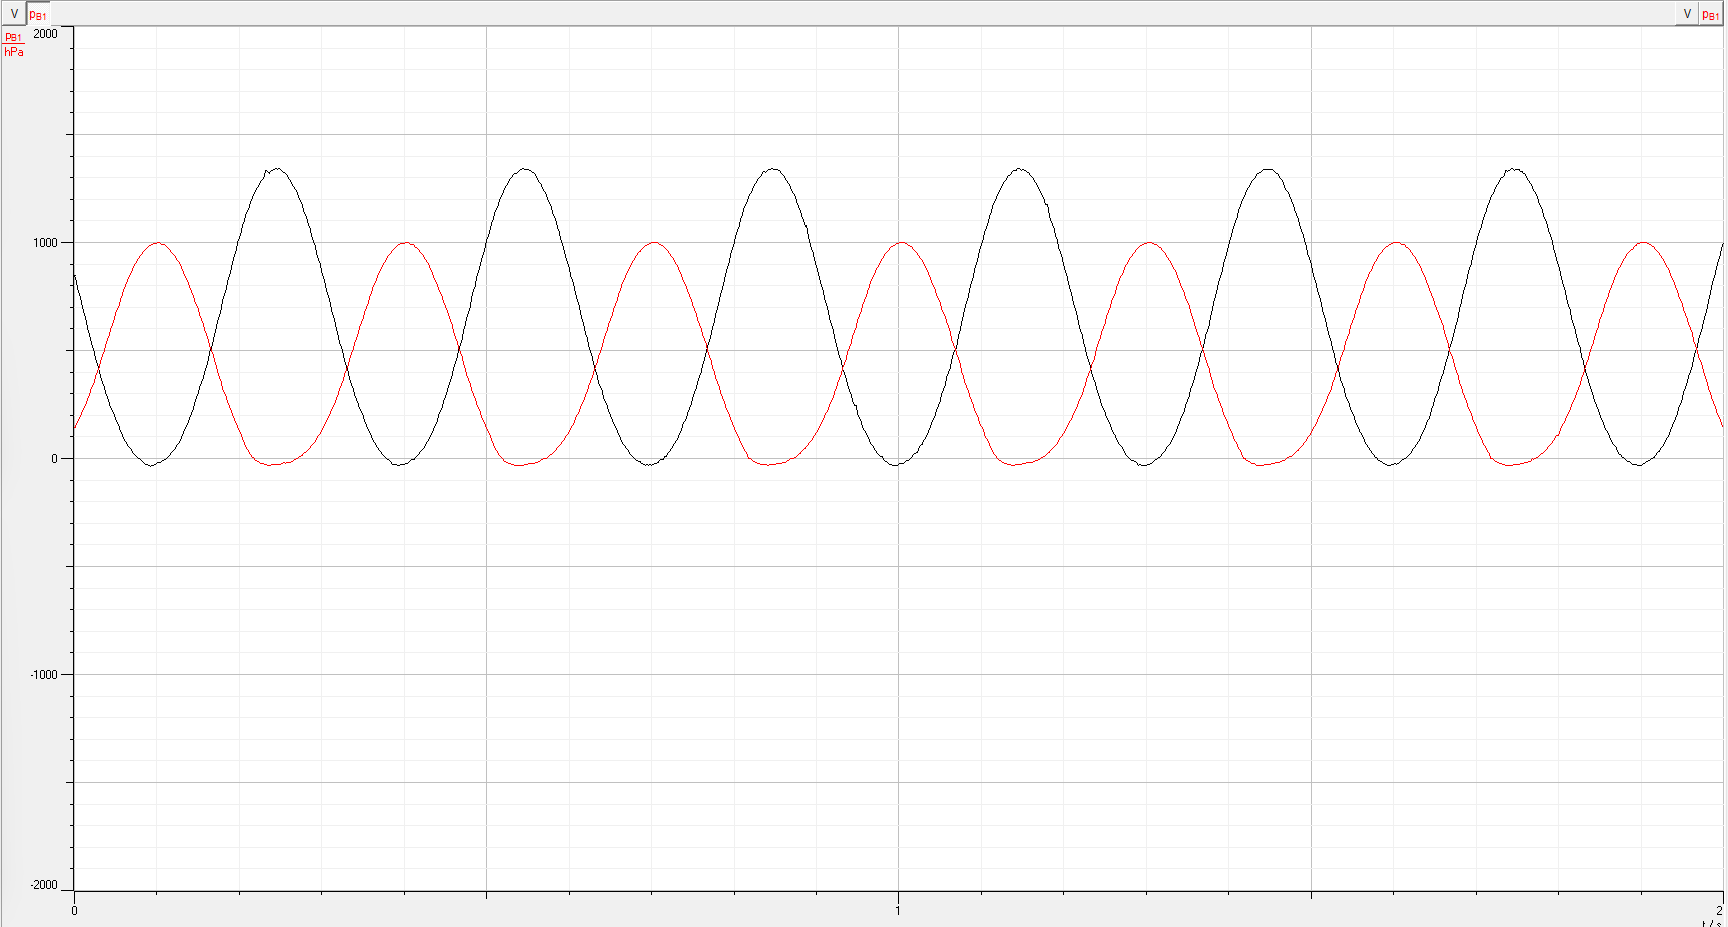
\includegraphics[scale=0.2]{f4}
    \end{center}
    \caption{Évolution de la pression (en rouge) et du volume (en noir) en fonction du temps}
\end{figure}
\begin{figure}[H]
    \begin{center}
        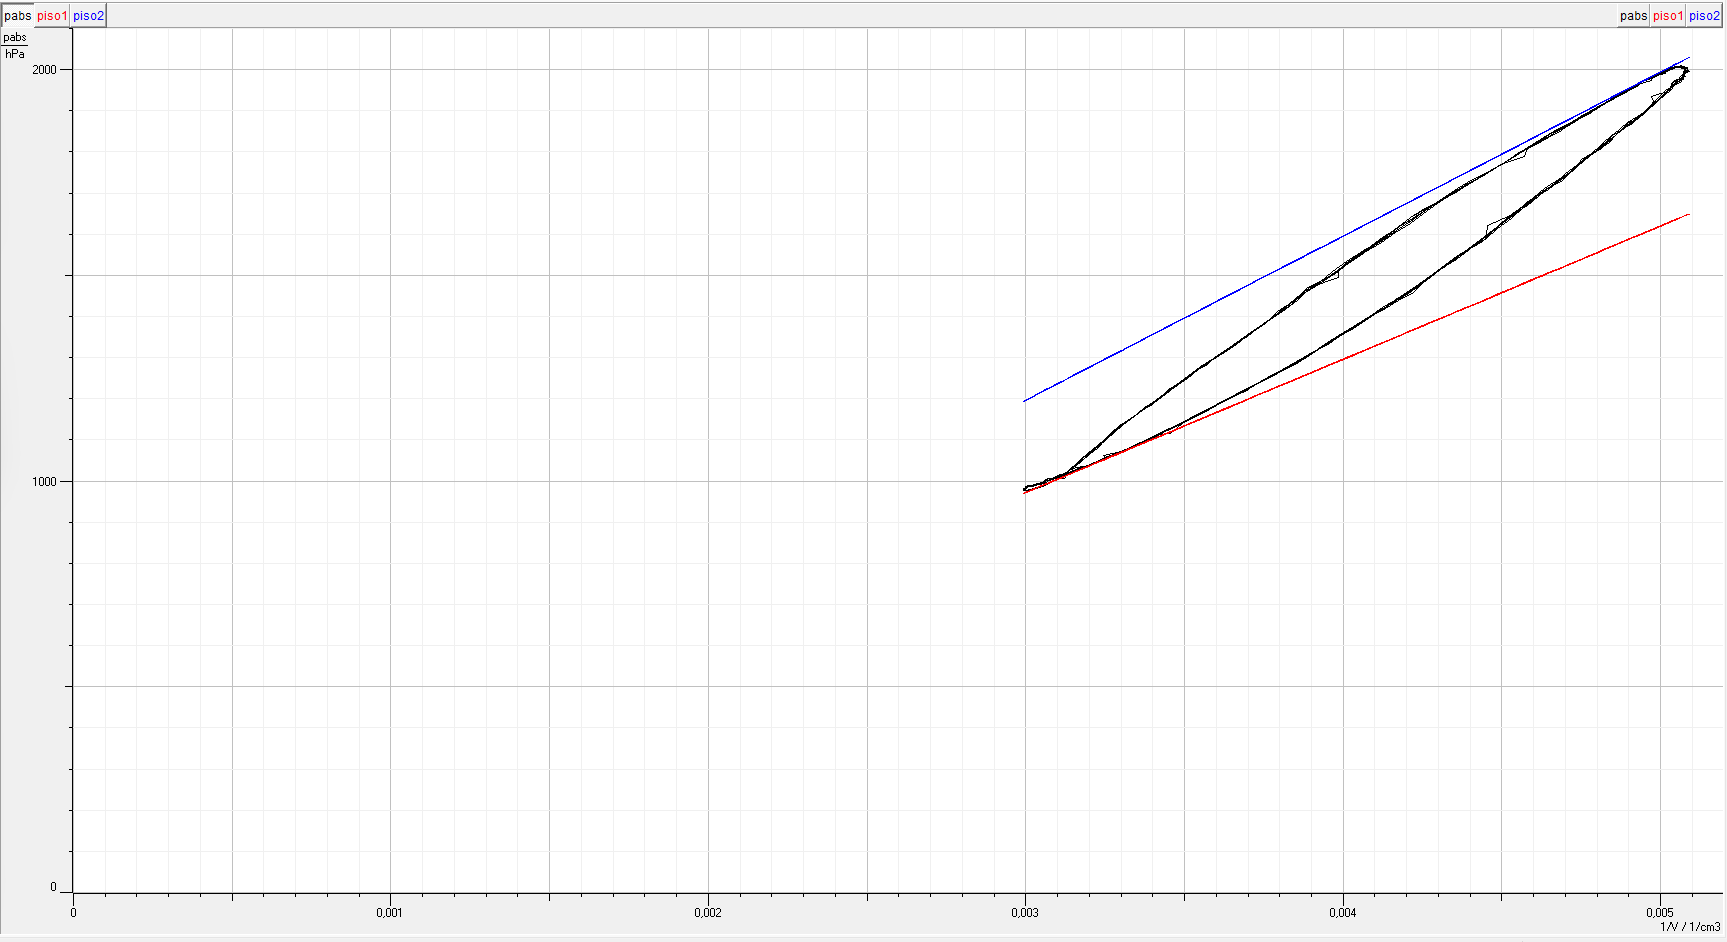
\includegraphics[scale=0.2]{f2}
    \end{center}
    \caption{Diagramme P en fonction de 1/V, sur lequel sont tracés les tangentes aux extramas de pression}
\end{figure}
\begin{figure}[H]
    \begin{center}
        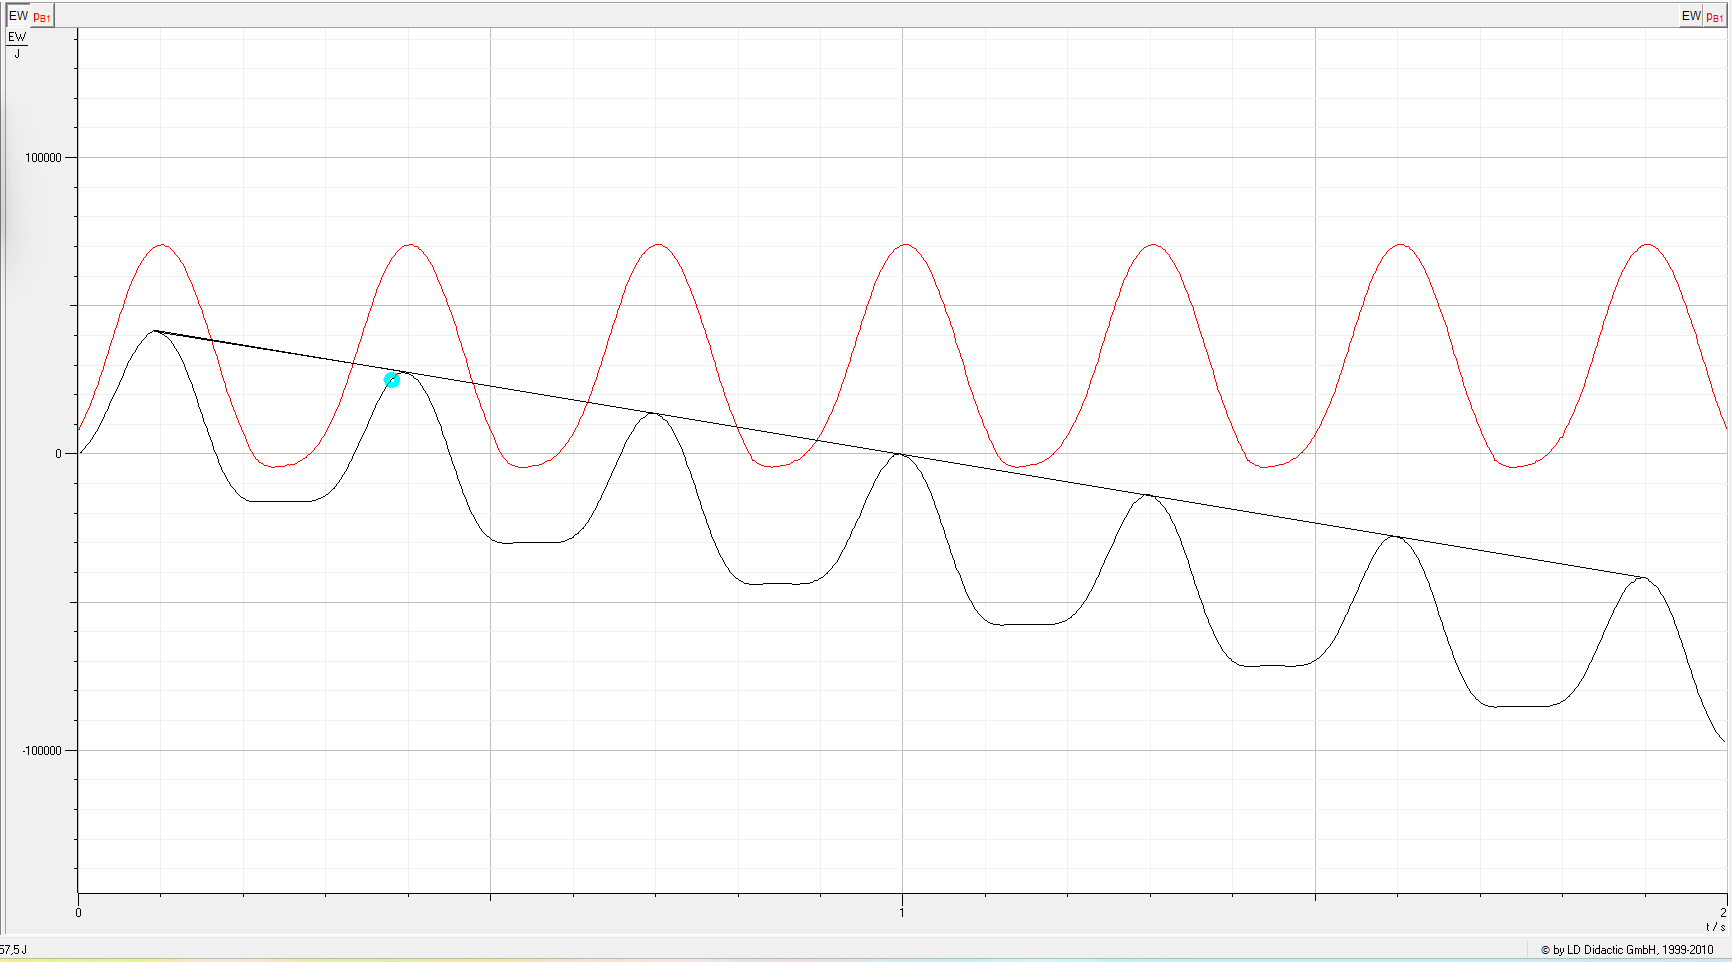
\includegraphics[scale=0.2]{f1}
    \end{center}
    \caption{Évolution de l'énergie du système EW en fonction du temps}
\end{figure}

\section{Exploitation des résultats}
\subsection{Détermination des grandeurs caractéristiques du cycle}

L'acquisition sur CASSY Lab permet de mesurer la période du cycle ainsi que les extrema de pression et de volume. Ces mesures sont essentielles pour le calcul du travail et des bilans de puissance.


Pour minimiser l'erreur de lecture, la durée de 6 cycles a été mesurée : $6\tau = 1805 \pm 5$ ms.
On en déduit la période : $\tau = \frac{1805}{6} \approx 300,8 \text{ ms (soit } 0,301 \text{ s)}$.


On note $P_{atm} = 1013$ hPa la pression atmosphérique au moment de l'expérience. Les pressions absolues sont calculées selon la relation $P_{abs} = P_{rel} + P_{atm}$.

\begin{table}[H]
\centering
\begin{tabular}{|l|c|c|c|}
\hline
{État du fluide} & {Pression relative} (hPa) & {Pression absolue} (hPa) & {Volume} (cm$^3$) \\ \hline
Point haut ($P_{max}$) & $+1052,0 \pm 1,0$ & 2065,0 & $195,0^*$ \\ \hline
Point bas ($P_{min}$) & $-84,7 \pm 1,0$ & 928,3 & 389,6 \\ \hline
\end{tabular}
\caption{Valeurs extrêmes de pression et de volume au cours du cycle en régime permanent.}
\end{table}
L'incertitude sur la pression absolue $u(P_{abs})$ est estimée à $2$ hPa (combinaison de l'incertitude du capteur et de la mesure atmosphérique). L'incertitude sur le volume dépend de la calibration du capteur de position, estimée à $u(V) \approx 5$ cm$^3$.
\subsection{Analyse du diagramme (P,V)}

Le cycle observé présente une forme décrite comme une "banane" courbée vers les hautes pressions. 
Il est parcouru dans le {sens horaire}. Dans ce sens, l'intégrale $\oint P dV$ est positive, ce qui implique que le travail reçu par le fluide $W = -\oint P dV$ est négatif. 
Le système fournit donc effectivement du travail au milieu extérieur.



L'aire délimitée par la courbe fermée représente la valeur absolue du travail utile produit par l'air au cours d'un cycle complet :
$$|W_{cycle}| = \int_{cycle} P dV$$
Plus cette aire est importante, plus l'énergie mécanique récupérée par cycle est grande.

L'observation du tracé réel permet de nuancer le modèle théorique. En effet, le cycle expérimental ne présente aucune phase strictement isochore ($V=cste$) ni isobare ($P=cste$).
Meme si on a découpé le mouvement en 4 phases, il y a en réalité une variation simultannée de pression et volume tout au long du cycle. On ne peut donc pas oberserver ce type de transformations.
\subsection{Diagramme P, 1/V}
En considérant l'air comme un gaz parfait, l'équation d'état est $PV = nRT$. Dans le diagramme $(P, 1/V)$, une transformation isotherme ($T = \text{cste}$) suit l'équation :
$$P = (nRT) \cdot \frac{1}{V}$$
Il s'agit de l'équation d'une droite de type $y = kx$ avec $x = 1/V$ et une pente $k = nRT$. 
L'{ordonnée à l'origine} de ces isothermes est théoriquement nulle ($P = 0$ lorsque $1/V = 0$, soit pour un volume infini).

Nous avons ajusté deux droites isothermes passants par l'origine, tangentes au cycle aux points de pression extrêmes :
\begin{itemize}
    \item Pour $P_{max}$ (tangente supérieure) : $k_{max} = nRT_{chaud} = 324\,000 \text{ hPa.cm}^3$
    \item Pour $P_{min}$ (tangente inférieure) : $k_{min} = nRT_{froid} = 198\,800 \text{ hPa.cm}^3$
\end{itemize}



On observe que le cycle réel ne suit pas ces droites sur des portions significatives. Le cycle est "inscrit" entre ces deux isothermes. Cela montre que les phases de détente et de compression ne sont pas purement isothermes : la température du gaz varie continuellement entre $T_{froid}$ et $T_{chaud}$ à mesure que le régénérateur déplace l'air.

On peut en déduire le rapport des températures.

$$\lambda = \frac{198\,800}{324\,000} \approx 0,613$$

Ce rapport, inférieur à 1, montre que la température absolue du gaz lors de la phase froide représente environ $61\%$ de sa température lors de la phase chaude. Ce paramètre est essentiel pour estimer l'efficacité théorique du cycle, car il est directement lié au gradient de température imposé par les sources.
\subsection{Calcul du travail mécanique}

Le travail est déterminé à partir de la puissance instantanée $PW = -p \cdot \frac{dV}{dt}$. La variable $EW$ calculée par CASSY Lab correspond à l'intégrale temporelle de cette puissance : $EW = \int PW \, dt$.

Les données brutes de CASSY utilisent des unités non-SI (hPa pour la pression et cm$^3$ pour le volume). Pour obtenir un travail en Joules (J), il est nécessaire d'appliquer les facteurs de conversion suivants :
\begin{itemize}
    \item $1 \text{ hPa} = 100 \text{ Pa}$ (soit $10^2$ kg.m$^{-1}$.s$^{-2}$)
    \item $1 \text{ cm}^3 = 10^{-6} \text{ m}^3$
\end{itemize}
Le produit $(P \cdot V)$ en unités brutes doit donc être multiplié par $10^2 \cdot 10^{-6} = {10^{-4}}$ pour obtenir des Joules.


La mesure totale sur $n = 6$ cycles donne $W_{total, \text{brut}} = -83\,357,5$ (unités CASSY).
Le travail SI pour l'ensemble des 6 cycles est :
$$W_{total, \text{SI}} = -83\,357,5 \cdot 10^{-4} \approx -8,336 \text{ J}$$

Le travail fourni par le fluide au cours d'un seul cycle est donc :
$$W = \frac{W_{total, \text{SI}}}{6} = \frac{-8,336}{6} \approx -1,389 \text{ J}$$


La valeur de $W$ est négative : le gaz fournit effectivement de l'énergie mécanique au milieu extérieur (le volant d'inertie).

\subsection{Synthèse des résultats}
\begin{table}[H]
\centering
\begin{tabular}{|l|c|l|}
\hline
{Grandeur} & {Symbole} & {Valeur et unité} \\ \hline
Tension filament & $U$ & $12,2 \pm 0,1$ V \\ \hline
Intensité filament & $I$ & $11,5 \pm 0,1$ A \\ \hline
Période du cycle & $\tau$ & $0,301 \pm 0,001$ s \\ \hline
Pression minimale (Absolue) & $P_{min}$ & $928,3$ hPa \\ \hline
Pression maximale (Absolue) & $P_{max}$ & $2065,0$ hPa \\ \hline
Rapport des températures (Gaz) & $\lambda$ & $0,613$ \\ \hline
Travail mécanique par cycle & $W$ & $-1,389 \pm 0,03$ J \\ \hline
Débit massique d'eau & $D_m$ & $(4,39 \pm 0,04) \cdot 10^{-3}$ kg.s$^{-1}$ \\ \hline
Température entrée eau & $T_e$ & $29,0 \pm 0,1$ $^{\circ}$C \\ \hline
Température sortie eau & $T_s$ & $32,5 \pm 0,1$ $^{\circ}$C \\ \hline
\end{tabular}
\caption{Synthèse des mesures expérimentales en régime permanent.}
\end{table}

\subsection{Bilan thermique}
\subsubsection{Source froide ($Q_F$)} 
La chaleur cédée par le gaz à l'eau de refroidissement au cours d'un cycle est calculée par :
$Q_F = D_m \cdot c_{eau} \cdot (T_s - T_e) \cdot \tau$
Avec $c_{eau} = 4180$ J.kg$^{-1}$.K$^{-1}$. 
D'après nos valeurs : 
$Q_F = 4,39 \cdot 10^{-3} \cdot 4180 \cdot (32,5 - 29,0) \cdot 0,301 \approx 19,33$ J.
Le transfert pour le gaz est donc : {$Q_F \approx -19,33$ J / cycle}.

\subsubsection{Source chaude ($Q_c$)} 
D'après le premier principe de la thermodynamique appliqué à un cycle ($\Delta U = 0$) :
$W + Q_c + Q_F = 0 \implies Q_c = - (W + Q_F)$
$Q_c = - (-1,389 - 19,33) \approx {20,72}$ {J / cycle}.

\subsubsection{Comparaison avec l'énergie Joule ($Q_{Joule}$)} 
L'énergie totale dissipée par le filament par cycle est :
$Q_{Joule} = U \cdot I \cdot \tau = 12,2 \cdot 11,5 \cdot 0,301 \approx {42,23}$ {J / cycle}.

On constate que $Q_{Joule} > Q_c$. La différence ($42,23 - 20,72 = 21,51$ J) représente les pertes thermiques du moteur vers l'environnement.

\subsection{Efficacité énergétique}

\subsubsection{Efficacité réelle ($\eta_M$)}
Elle représente le rapport entre le travail utile produit et la chaleur réellement absorbée par le gaz :
$$\eta_M = \frac{|W|}{Q_c} = \frac{1,389}{20,72} \approx {6,70\%}$$

\subsubsection{Efficacité de Carnot ($\eta_C$)}
C'est l'efficacité maximale théorique d'un moteur ditherme opérant entre les températures extrêmes du gaz ($T_F$ et $T_C$). En utilisant le rapport $\lambda = T_F / T_C \approx 0,613$ identifié sur le diagramme $(P, 1/V)$ :
$$\eta_C = 1 - \lambda = 1 - 0,613 = {38,7\%}$$



L'efficacité réelle ($\approx 6,7\%$) est nettement inférieure à l'efficacité de Carnot. Cet écart peut être dû aux irréversibilités (comme les frottements du piston, pertes liées aux régénérateur) et au fait que le cycle réel n'est pas composé d'isothermes parfaits (comme on l'a vu en figure 3). 
\section{Conclusion}
Ce TP a permis de valider le fonctionnement du moteur Stirling. Malgré des pertes thermiques importantes (différence entre $Q_{Joule}$ et $Q_c$), le dispositif convertit efficacement une partie de la chaleur en travail mécanique. Le régénérateur est l'organe clé permettant d'augmenter l'efficacité en stockant temporairement l'énergie interne du gaz lors des phases de transfert.

\end{document}